\section*{Part E: Introduction to FEM (Unit 5)}
\addcontentsline{toc}{section}{Part E: Introduction to FEM}

\paragraph{1. Three key steps from physics to a numerical discretization.}
\begin{enumerate}[nosep,leftmargin=1.6em]
\item \textbf{Mathematical model (strong form).} Capture the physics as a governing PDE plus its
boundary and initial conditions: the exact, continuous description.
\item \textbf{Weak / variational form.} Multiply by a test function and integrate over the domain,
moving derivatives onto the test function. This relaxes the continuity requirement and is what makes
the problem amenable to piecewise approximation.
\item \textbf{Discretization (Galerkin).} Mesh the domain into finite elements, expand the unknown in
a finite set of basis (shape) functions, and assemble the result into an algebraic system
$\mathbf{K}\mathbf{u}=\mathbf{f}$ that a computer solves; then post-process and check convergence.
\end{enumerate}

\paragraph{2. Ideal polynomial order of the basis functions.}
\textbf{Quadratic (second-order) elements} are usually the sweet spot.
\begin{itemize}[nosep,leftmargin=1.6em]
\item \emph{Lower order} (linear/hat functions) is cheap and robust and represents straight fields
exactly, but it only captures curvature crudely, so smooth or high-gradient fields need a very fine
mesh to reach the same accuracy.
\item \emph{Higher order} (cubic and up) gives excellent accuracy per element and resolves curvature
with few elements, but the cost per element climbs, matrices become denser and worse-conditioned, and
high orders can oscillate (Runge-type wiggles) near sharp features.
\end{itemize}
Quadratic elements capture curvature well while keeping the cost and conditioning manageable, which
gives the best accuracy per unit effort for typical smooth problems.

\paragraph{3. Qualitative grid spacing for linear (hat) basis functions.}
Linear hat functions reproduce a straight line \emph{exactly}, so the rule is simple: \textbf{use a
coarse spacing on straight parts, refine where the curvature is high, and always place a node at every
corner/kink} (where the slope is discontinuous).
\begin{itemize}[nosep,leftmargin=1.6em]
\item \textbf{(a) Straight line:} one element (two nodes) is enough, since it is exact.
\item \textbf{(b) Exponential:} a graded mesh, fine where the function bends sharply and progressively
coarser in the flat tail.
\item \textbf{(c) Mixed curve:} coarse on the straight segments and the triangular peak (with nodes at
the joints $x=-4,-2,2,4,6$), but densely spaced across the high-curvature semicircle.
\end{itemize}

\begin{figure}[H]
\centering
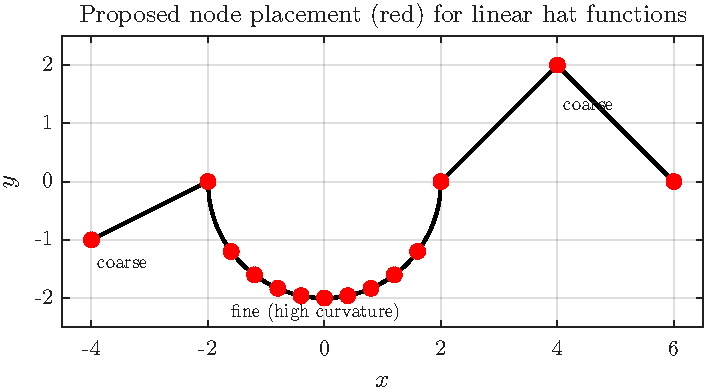
\includegraphics[width=0.66\textwidth]{figures/fem_grid.pdf}
\caption{Proposed node placement (red) for curve (c): coarse on the straight pieces, dense across the
curved semicircle, with nodes pinned at every kink.}
\label{fig:femgrid}
\end{figure}
